% tests
% https://codoid.com/data-quality-checks-data-warehouse-etl/
% more tests
% https://codoid.com/etl-data-quality-testing-best-practices/

Once the source database has been migrated to the Cloud, it is important to verify the correctness of the data contained in it.
Having wrong information may cause poor business decisions, as well as other issues.

A wide array of tests can be performed on a Data Warehouse to assess the correctness of the data it contains \cite{bib:related_work:tests:tests1, bib:related_work:tests:tests2}.

Most state-of-the-art tests, however, are not suited for the energy market domain, due to the nature of the data required.

We will now analyze some of the various data quality tests widely used in the world, providing a final comparison between state-of-the-art testing techniques and the particular requirements of the energy market domain.

\subsection{Test Types}
    \paragraph{Data type coherency}
        \begin{figure}
            \centering
            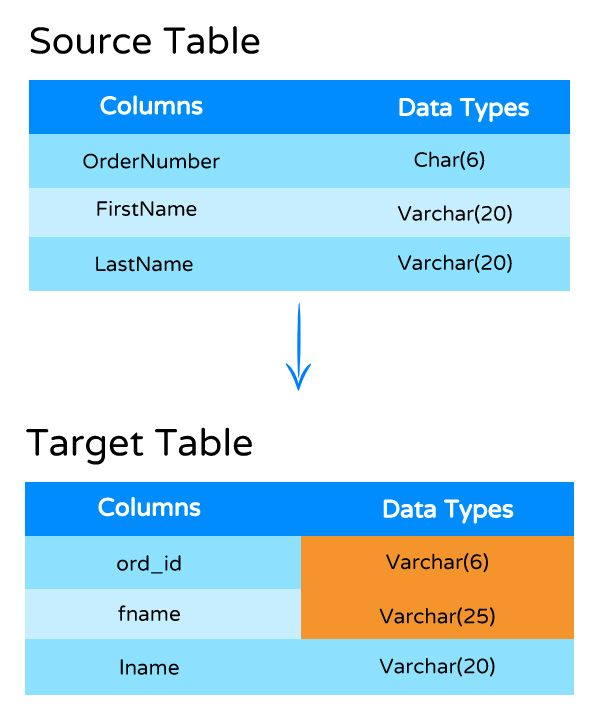
\includegraphics[width=.5\textwidth]{res/relatedwork/data_type.jpg}
            \caption{Different data types during migration.}
            \label{fig:related:tests:data_type}
        \end{figure}
        
        When performing a migration, it is important to pay attention to the format chosen for the table, not only in terms of table structure but also regarding data types used for each field.
        
        As we can see from Figure \ref{fig:related:tests:data_type}, it is possible to have mismatches between the source and destination tables.
        
        This can lead to unexpected problems.
        For example, if a \texttt{VARCHAR} field supports less characters on the destination table, the string may get truncated.
        
    \paragraph{NULL values}
        Some columns are not supposed to contain \texttt{NULL} values.
        
        It is important to make sure that any \texttt{Not NULL} constraints are respected, both by reproducing the constraint in the destination table and by specifically looking for \texttt{NULL} values.
        
        The presence of \texttt{NULL} values is often indicative of problems in the ETL process.
    
    \paragraph{Duplicate records}
        Another important test is controlling whether the destination table contains any duplicate entries where it's not supposed to, such as IDs.
        
        Having multiple instances of the same record may result in inaccurate results, leading to poor business decisions.
    
    \paragraph{Orphan records}
        \begin{figure}
            \centering
            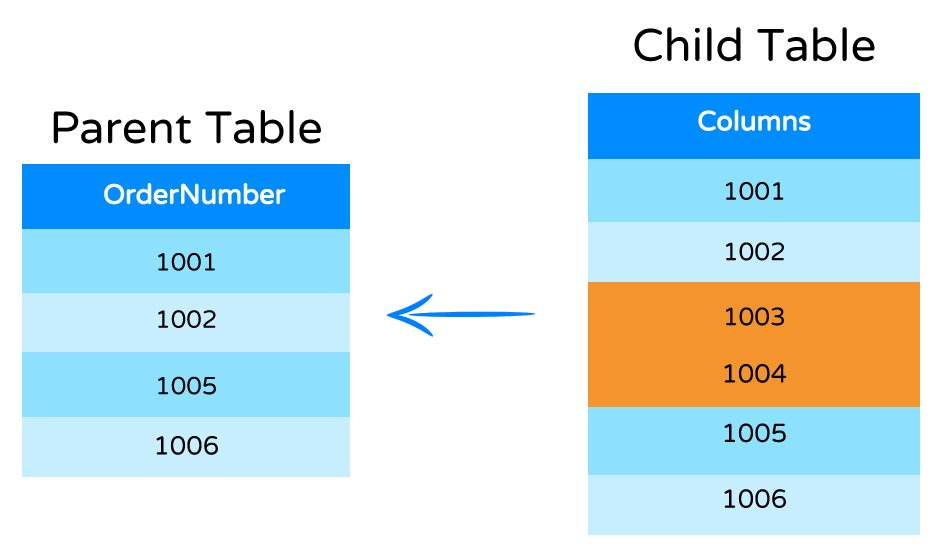
\includegraphics[width=.5\textwidth]{res/relatedwork/orphan_records.jpg}
            \caption{Orphan records.}
            \label{fig:related:tests:orphan}
        \end{figure}
        
        Orphan records are often indicative of missing data or problems in the ETL process.
        
        An orphan record can be define as an incomplete foreign key: on a child table we have an ID which doesn't appear in the parent table.
        For example, we may have billing information for a specific user, but no information about the user himself.
        
        Figure \ref{fig:related:tests:orphan} shows an example of orphan records.
        
    \paragraph{Unknown data}
        If possible, it is also a good idea to make sure values are between a reasonable range.
        
        For example, having a client over 150 years old is surely indicative of some problems.
        The same can be said for negative ages.
        
        This test can however only be applied on specific types of information: in some cases all possible values may be acceptable, such as profits or losses generated from a particular energy plant.
    
    \paragraph{Min/max validations}
        Min/max validation can assess the range of particular kinds of data.
        
        Having different ranges between the two databases can indicate either missing data (if the range is too small), or unexpected data (if the range on the cloud exceeds the local one).
    
    \paragraph{Timeliness}
        The same information may change in time.
        Downloading the same information in two different moments may give different results, if that value is updated over time.
        
        When performing a migration, it is important to pay attention to these different versions and to retrieve the correct one.
        
    
\subsection{Energy Market Domain Issues}
    Some of the tests described above are not suited for the energy market domain for a variety of reasons.
    
    \paragraph{Forecast updates}
        Energy forecasts are often updated, meaning that \textit{Timeliness} test types would fail.
        
        However, this is not a problem, since more recent versions are more accurate and are the only ones actually needed.
        
        As a consequence, these tests cannot be applied on this kind of data.
    
    \paragraph{Date ranges}
        The local database contains some data related to several years ago, which are no longer needed by any user.
        
        As such, \textit{min/max validation} tests need to be slightly tweaked.
        Instead of comparing the exact ranges, the cloud is allowed have less data, as long as these information are very old.
        
    \paragraph{Unexpected data values}
        For most values used in the energy market domain, all possible values are acceptable.
        Values outside of an ``expected'' range may indeed be indicative of unexpected market events and must as such be treated as correct.
        
        This kind of tests, as a consequence, cannot be applied on this particular process.

    